%%%%%%%%%%%%%%%%%%%%%%%%%%%%%%%%%%%%%%%%%%%%%%%%%%%%%%%
%                  File: OPTICAmeetings.tex           %
%                  Date: 31 July 2023                 %
%                                                     %
%     For preparing LaTeX manuscripts for submission  %
%     submission to Optica meetings and conferences   %
%                                                     %
%         (c) 2018-2022 Optica Publishing Group       %
%%%%%%%%%%%%%%%%%%%%%%%%%%%%%%%%%%%%%%%%%%%%%%%%%%%%%%%

\documentclass[article,11 pt]{article} 
\usepackage{times}
\usepackage{float}
\setlength{\baselineskip}{1.5\baselineskip}
%% if A4 paper needed, change letterpaper to A4

\usepackage{opticameet3} %% use version 3 for proper copyright statement

%% provide authormark
\newcommand\authormark[1]{\textsuperscript{#1}}

%% standard packages and arguments should be modified as needed
\usepackage{amsmath,amssymb}
\usepackage[colorlinks=true,bookmarks=false,citecolor=blue,urlcolor=blue]{hyperref} %pdflatex
%\usepackage[breaklinks,colorlinks=true,bookmarks=false,citecolor=blue,urlcolor=blue]{hyperref} %latex w/dvipdf
\usepackage{matlab-prettifier}
\usepackage{tabularx}
\usepackage{titling}
\renewcommand{\tablename}{Tabla}

\usepackage{fancyhdr} % Paquete para personalizar encabezados y pies de página
\pagestyle{fancy} % Activar encabezado y pie de página personalizados
\fancyhf{} % Limpiar configuraciones previas
\fancyfoot[C]{\thepage} % Mostrar número de página centrado en el pie de página


\begin{document}

\title{Problem Set 1: Big Data \& Machine Learning}

% \author{Author name(s)}
% \address{Author affiliation and full address}
% \email{e-mail address}
%%Uncomment the following line to override copyright year from the default current year.
%\copyrightyear{2024}

\author{Juan Esteban Díaz Torres\authormark{1}, Natalia Plata Ángel \authormark{2} y Ángel David Ramírez Torres \authormark{3} }

\address{\authormark{1} 202020319
\authormark{2} 202013152 
\authormark{3} 202112704 }

\href{https://github.com/angelramirez63/Problem-Set-1}{Repositorio}.

%\email{\authormark{*}opex@optica.org} %% email address is required



%\begin{abstract}
%\LaTeX{} users preparing manuscripts for Optica meetings or conferences
%should use  the \texttt{opticameet3.sty} style file and should observe these
%guidelines to adhere to Optica requirements. Users of Bib\TeX{} may use the \texttt{opticajnl.bst} style file, which is included in this distribution. Comments and questions should be directed to the Optica Conference Papers staff (cstech@opg.org).
%\end{abstract}

\section{Introducción}

En los últimos 20 años, Colombia ha aprobado 12 reformas tributarias, lo que equivale a una cada 1,7 años en promedio (Casas, 2024). La frecuencia con la que se implementan estas reformas refleja las crecientes necesidades de financiamiento del Estado colombiano para cumplir con sus obligaciones. En este contexto, Mejía (2022) recomienda adoptar medidas para reducir la evasión fiscal, que según sus estimaciones equivale al 5,4\% del PIB, de los cuales el 0,7\% corresponde a la evasión del impuesto de renta de personas naturales. Una de las principales barreras para avanzar en la lucha contra la evasión es la limitada adopción de herramientas tecnológicas de gestión para su detección y combate. Para abordar este desafío, los modelos de predicción de ingresos podrían ser una herramienta clave para identificar evasores, mejorar la eficiencia operativa del Estado y, en última instancia, fortalecer el recaudo tributario. 
\\
\\
En este contexto, el presente trabajo pretende realizar un acercamiento a la modelación del salario y su predicción. Los datos empleados provienen de la Gran Encuesta Integral de Hogares (GEIH), que contiene información de condiciones laborales, ingresos y otras características de miles de colombianos en contextos urbanos.La muestra se limitó a los individuos ocupados y mayores de edad, con un total de 9,848 observaciones y 105 variables al final de la limpieza.
\\
\\
En este trabajo se analizó la dinámica entre salario y edad encontrando que la edad tiene un efecto marginal decreciente sobre el salario. Se estima que el salario tiene un pico alrededor de los 44 años de edad. Por otra parte, se analizó la brecha salarial por género, encontrando que el efecto de ser mujer sobre el salario es negativo. Algunas explicaciones plausibles para este fenómeno son la carga desproporcionada de la economía del cuidado que recae sobre las mujeres y la penalización a la maternidad. Es importante resaltar que con los datos disponibles no podemos hacer afirmación de tipo causal. Por último, se evaluó el desempeño. predictivo de los modelos anteriormente descritos y otros adicionales. En cuanto al desempeño predictivo de los modelos planteados, el modelo con mejor ajuste presentó un error de predicción de 1.5 pesos aproximadamente. Este error representa el 0.02\% del valor promedio del salario por hora que es de 8,116 pesos. Este modelo incluía variables como la formalidad, edad, género, experiencia, estrato, subsidios y bonificaciones. Además, se analizó el \textit{trade-off} entre sesgo y varianza, identificando que aquellos modelos con demasiada o muy poca flexibilidad (varianza) tienen peor desempeño que aquellos más balanceados.

\section{Descripción de los datos}
\subsection{Fuente}

Los datos empleados en este trabajo provienen de la Gran Encuesta Integral de Hogares (GEIH) realizada por el Departamento Administrativo Nacional de Estadística (DANE) la cual se realiza para capturar información sobre las condiciones de empleo, ingresos y otras características de la población colombiana. Específicamente, se utilizaron datos del reporte de “Medición de Pobreza Monetaria y Desigualdad” del año 2018. 

\subsection{Obtención}
Estos dátos fueron obtenidos a por medio de \textit{webscrapping}, ya que estaban contenidos en una página web en forma de tablas. Inicialmente, existía una restricción para acceder a ellos, dado que no se encontraban en el enlace visible al interactuar directamente con la página. Esto se debía a que la página web cargaba la información desde otra fuente. Por esta razón, fue necesario inspeccionar el código HTML para identificar el enlace correcto donde se alojaban las tablas de datos.
\\
\\
Adicionalmente, la información estaba distribuida en diez \textit{Data Chunks} o secciones ubicadas en distintos enlaces dentro del sitio web original. Para extraer todos los datos, fue necesario iterar sobre las distintas páginas. Con este propósito, se diseñó un proceso iterativo que recopilaba cada sección desde su respectivo enlace y las integraba en una base de datos. La base de datos obtenida con este método contenía 32.177 observaciones y 178 variables.

\subsection{Procesamiento}
 Antes de utilizar la base de datos para modelar el salario, fue necesario realizar un proceso de depuración. Primero, se filtró la base de datos para conservar únicamente a los individuos ocupados y mayores de 18 años, dado que el objetivo del análisis es modelar el ingreso salarial. Adicionalmente, se excluyeron las observaciones con valores faltantes en la variable salario. Este filtro resultó en la eliminación de personas que trabajan por cuenta propia, para quienes suele ser difícil distinguir entre el ingreso laboral y las ganancias del negocio, debido a la ausencia de una contabilidad separada para ambos conceptos. Luego, se eliminaron aquellas variables que contenían únicamente valores faltantes o que tomaban el mismo valor en todas las observaciones, ya que no aportarían información relevante para mejorar la precisión de los modelos. Además, descartaron las variables con más del 60\% de valores faltantes, ya que su inclusión podría afectar significativamente a los modelos debido a la necesidad de imputación de datos.  
\\
\\
Después de este paso, se imputaron los valores faltantes de las variables restantes. Primero, las variables categóricas se completaron con la moda, es decir, la categoría más frecuente dentro de cada estrato y categoría de formalidad o informalidad. Esta elección se basa en la premisa de que las personas dentro de un mismo estrato suelen compartir contextos socioeconómicos similares. Además, estas variables se transformaron en factores para facilitar su inclusión en los modelos. Posteriormente, el resto de las variables se imputaron utilizando el método de K-Nearest Neighbors (KNN), el cual mide la similitud entre observaciones dentro de la base de datos e identifica los k vecinos más cercanos para cada una. A partir de estos vecinos, se completan los valores faltantes asignando aquellos presentes en las observaciones más similares.
\\
\\
Por otra parte, se aplicaron procedimientos para el tratamiento de valores atípicos y observaciones influyentes. Primero, se identificaron las variables relacionadas con el ingreso, cuya distribución suele presentar una acumulación hacia la izquierda y una alta dispersión hacia la derecha. Para estas variables, se determinó el percentil 97.5 y se reemplazaron con este valor aquellas observaciones que lo superaban. Además, se analizaron las observaciones influyentes en la relación entre salario y edad, eliminando las 10 con mayor influencia.
 
\subsection{Estadísiticas descriptivas}

En la Tabla \ref{tab:estadisticas_completas} se presentan las estadísticas descriptivas de la base de datos resultante tras el procesamiento de datos descrito previamente. Esta base cuenta con 9,848 observaciones.
\\
\\
En promedio, los individuos de la muestra tienen 36.17 años, un salario mensual de 1,609,575 pesos —más del doble del salario mínimo en Colombia para 2018, que era de 781,242 pesos— y un salario por hora de 8,111 pesos, con una jornada laboral de 48.36 horas semanales. En cuanto a las condiciones laborales, el empleo formal como trabajador dependiente predomina en la muestra. El 89\% de los individuos son empleados de una empresa privada, el 77\% reporta tener un empleo formal y el 52\% trabaja en empresas con más de 50 empleados. Por otro lado, la mayoría de los individuos están afiliados a los sistemas de seguridad social: el 76\% cotiza a pensión y el 89\% pertenece al régimen contributivo de salud. Además, el 45\% de la muestra ha cursado educación terciaria. En términos generales, la muestra anteriormente descrita tiene un mayor nivel educativo, mejores condiciones laborales y mayores ingresos que el colombiano promedio, lo cual puede estar explicado por el hecho de que la muestra proviene de un contexto urbano. 

\begin{table}[!htbp] 
    \centering 
    \caption{Estadísticas descriptivas: variables numéricas y categóricas} 
    \label{tab:estadisticas_completas} 

    \resizebox{0.8\textwidth}{!}{ % Ajusta el tamaño de la primera tabla
        \begin{tabular}{lccccc} 
            \hline 
            \hline \\[-1.8ex] 
            Variable & N & Media & Desv. Est. & Min & Max \\ 
            \hline \\[-1.8ex] 
            Salario mensual & 9,848 & 1,609,575 & 1,533,651 & 20,000 & 7,892,292 \\ 
            Salario por hora & 9,848 & 8,115.37 & 8,080.51 & 326.67 & 41,470.34 \\ 
            ln(Salario) & 9,848 & 8.71 & 0.69 & 5.79 & 10.63 \\ 
            Edad & 9,848 & 36.17 & 11.92 & 18 & 73 \\ 
            Sexo (1 = Mujer) & 9,848 & 0.50 & 0.50 & 0 & 1 \\ 
            Trabaja en microempresa (1 = Sí) & 9,848 & 0.23 & 0.42 & 0 & 1 \\ 
            Trabajo formal (1 = Sí) & 9,848 & 0.77 & 0.42 & 0 & 1 \\ 
            Horas trabajadas & 9,848 & 48.36 & 12.23 & 1 & 130 \\ 
            Segundo trabajo (1 = Sí) & 9,848 & 0.03 & 0.17 & 0 & 1 \\ 
            \hline 
            
        \end{tabular}
    }

    \vspace{0.2cm} % Espacio entre tablas
\\
    \resizebox{0.8\textwidth}{!}{ % Segunda tabla ocupa todo el ancho disponible
        \begin{tabular}{lcccc} 
            
            \hline \\[-1.8ex] 
            Variable & Categoría & Descripción & Frecuencia & Porcentaje \\ 
            \hline \\[-1.8ex] 
            Nivel educativo & 7 & Educación terciaria & 4,466 & 45.35 \\ 
            Tipo de empleo & 1 & Empleado de empresa particular & 8,717 & 88.52 \\ 
            Oficio & 39 & Apoyo administrativo y logístico & 813 & 8.26 \\ 
            Régimen de salud & 1 & Régimen contributivo & 8,745 & 88.80 \\ 
            Cotiza a pensión & 1 & Sí cotiza & 7,496 & 76.12 \\  
            Tamaño de empresa & 5 & $>$ 50 empleados& 5,093 & 51.72 \\ 
            \hline 
        \end{tabular} 
    }
\par{\footnotesize{\textit{Nota:} En el panel superior se pueden ver las estadísticas descriptivas de las variables numéricas continuas o variables categóricas binarias, para las que se puede interpretar el promedio. En el panel inferior se puede ver la categoría más frecuente para las variables categóricas con múltiples niveles.}}
        
\end{table} 
La Figura \ref{fig:salarios} presenta la distribución del salario por hora en pesos (panel izquierdo) y su transformación mediante el logaritmo natural (panel derecho). En la escala original, la distribución exhibe una alta concentración de individuos en los rangos salariales más bajos y una cola larga hacia valores superiores. La diferencia entre la media (línea azul) y la mediana (línea roja) sugiere la presencia de valores atípicos que elevan el promedio salarial. La transformación logarítmica, en contraste, reduce la asimetría y aproxima la distribución a una forma más normal. Esta transformación es particularmente útil en el análisis del mercado laboral, ya que permite evaluar cambios salariales en términos relativos y mitigar el impacto de valores extremos en los resultados. La concentración de salarios bajos observada en la distribución original resalta posibles desigualdades en la estructura salarial colombiana, lo que sugiere la necesidad de analizar factores como el acceso a educación y la formalidad laboral al modelar el salario.

\begin{figure}[h]
    \centering
    \caption{Distribución del salario por hora y su logaritmo natural}
    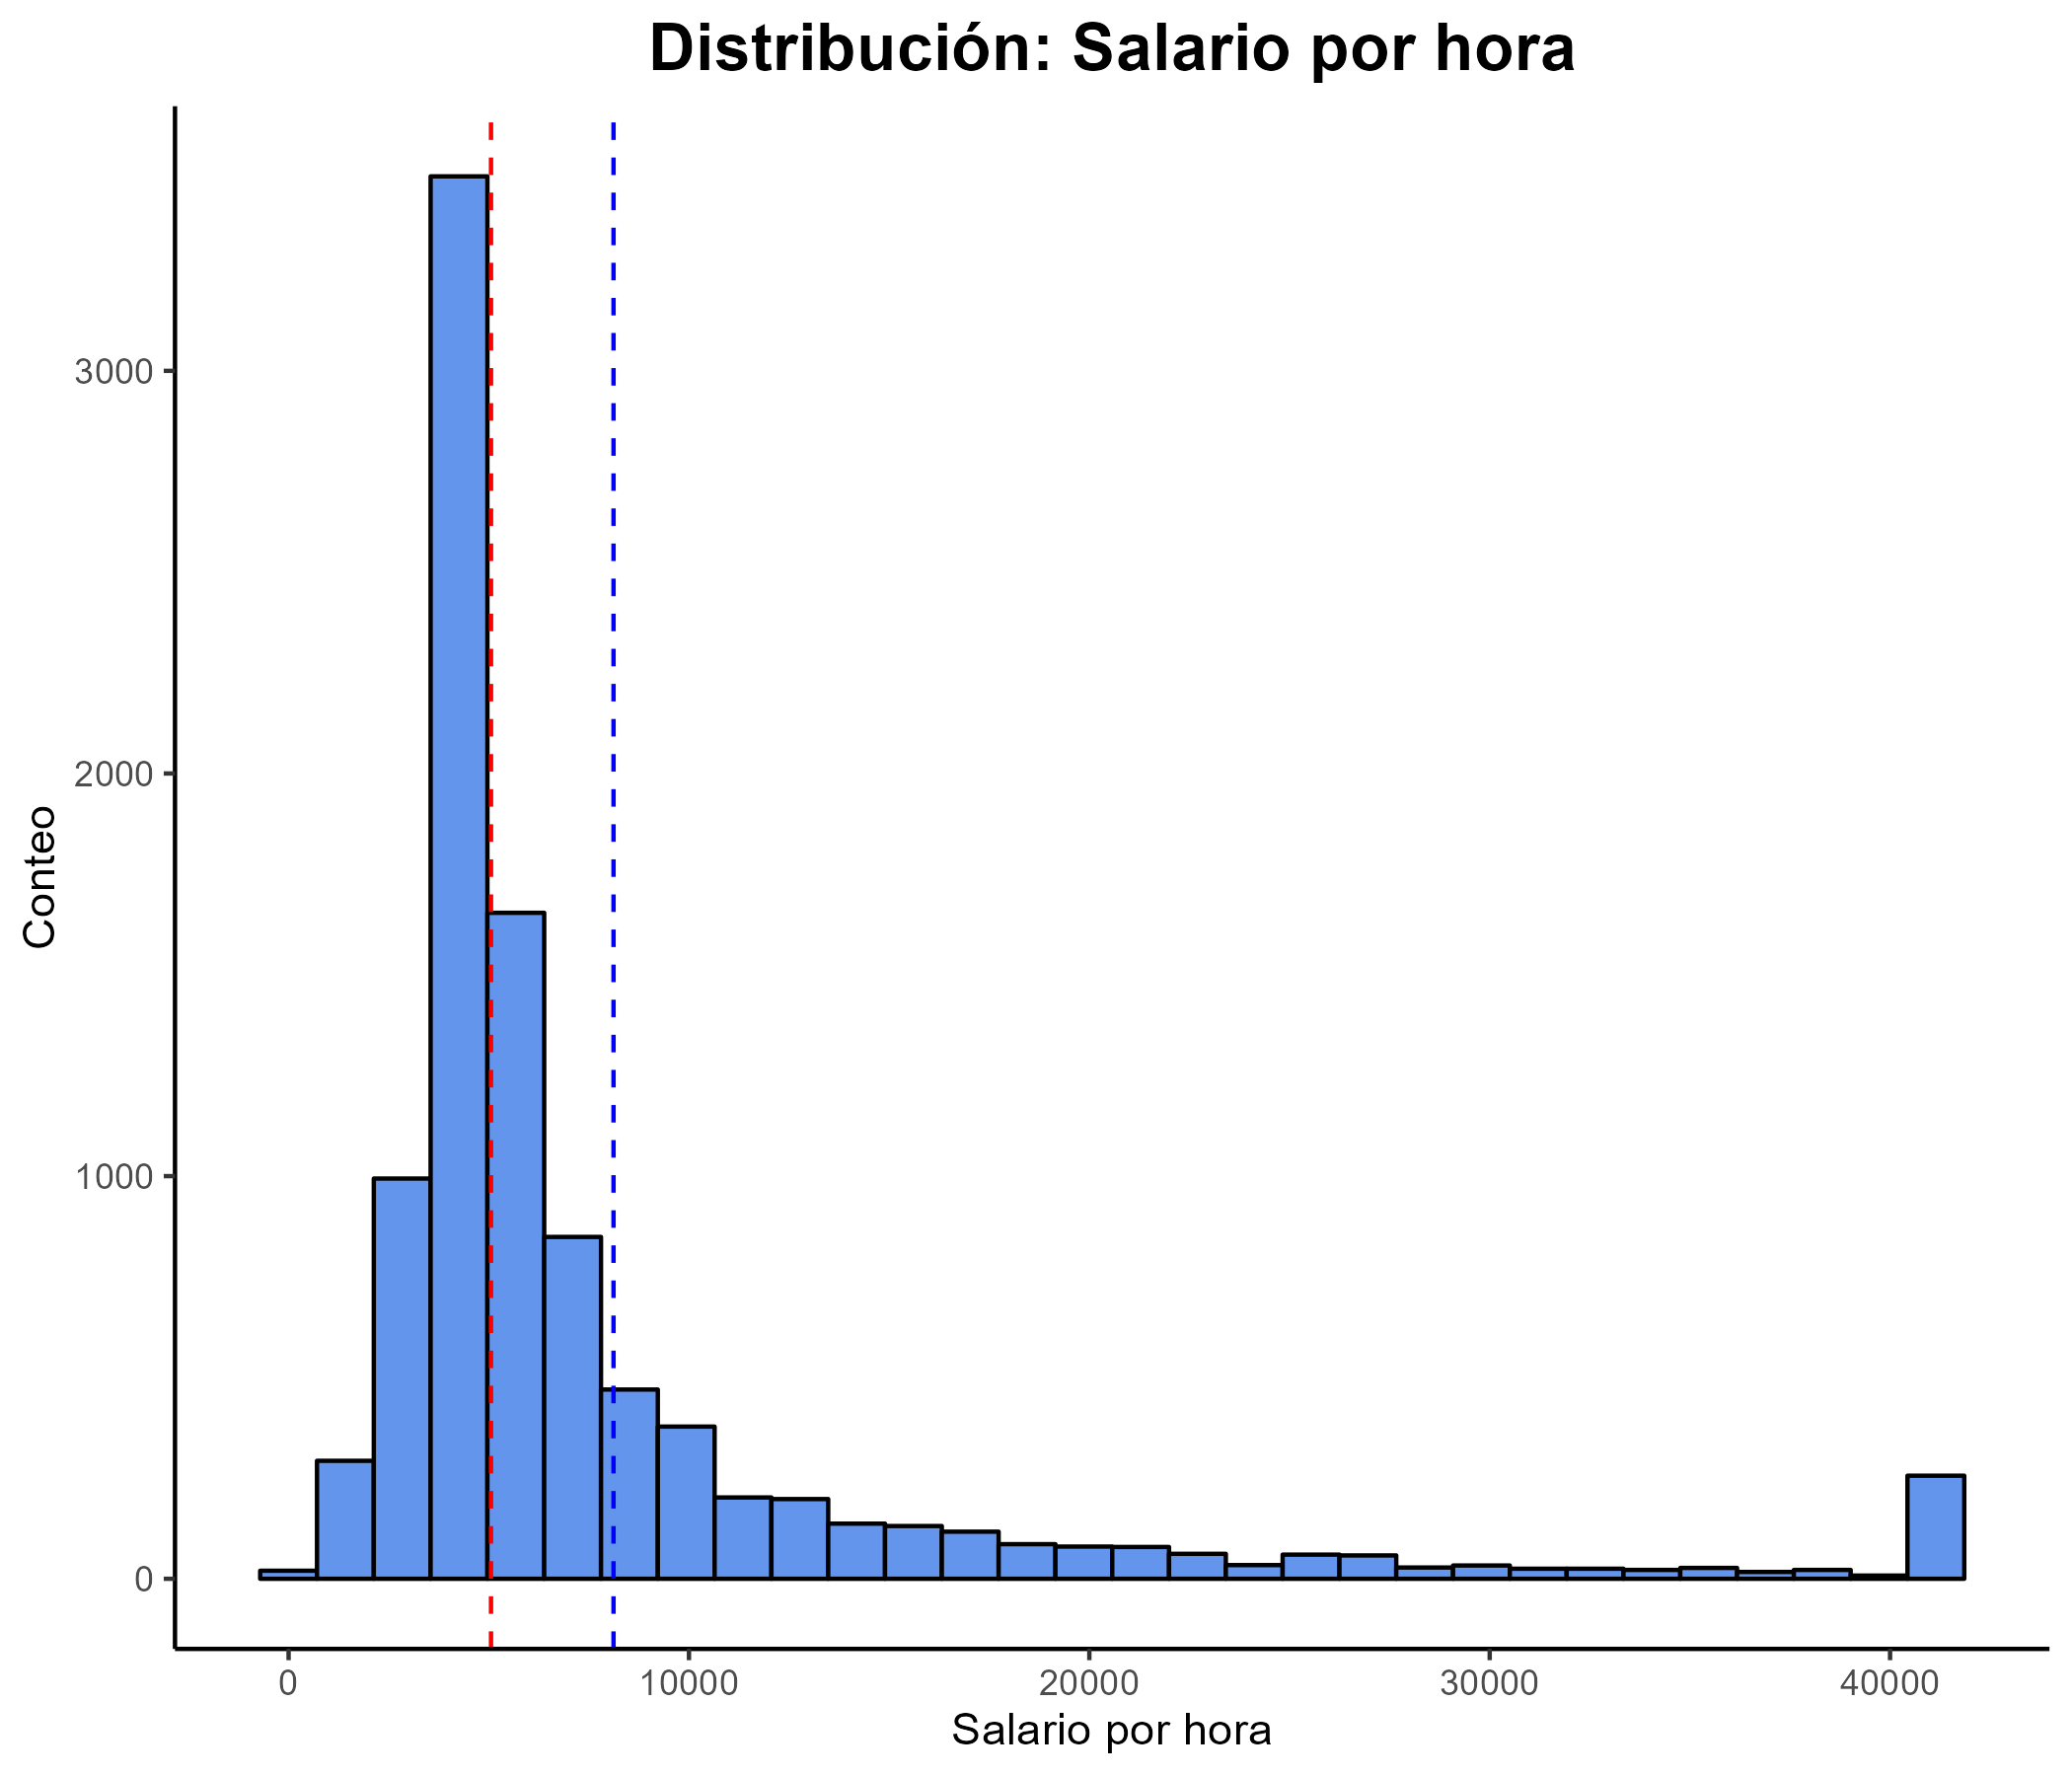
\includegraphics[width=0.45\textwidth]{Graficos/y_ingLab_m_ha.png}
    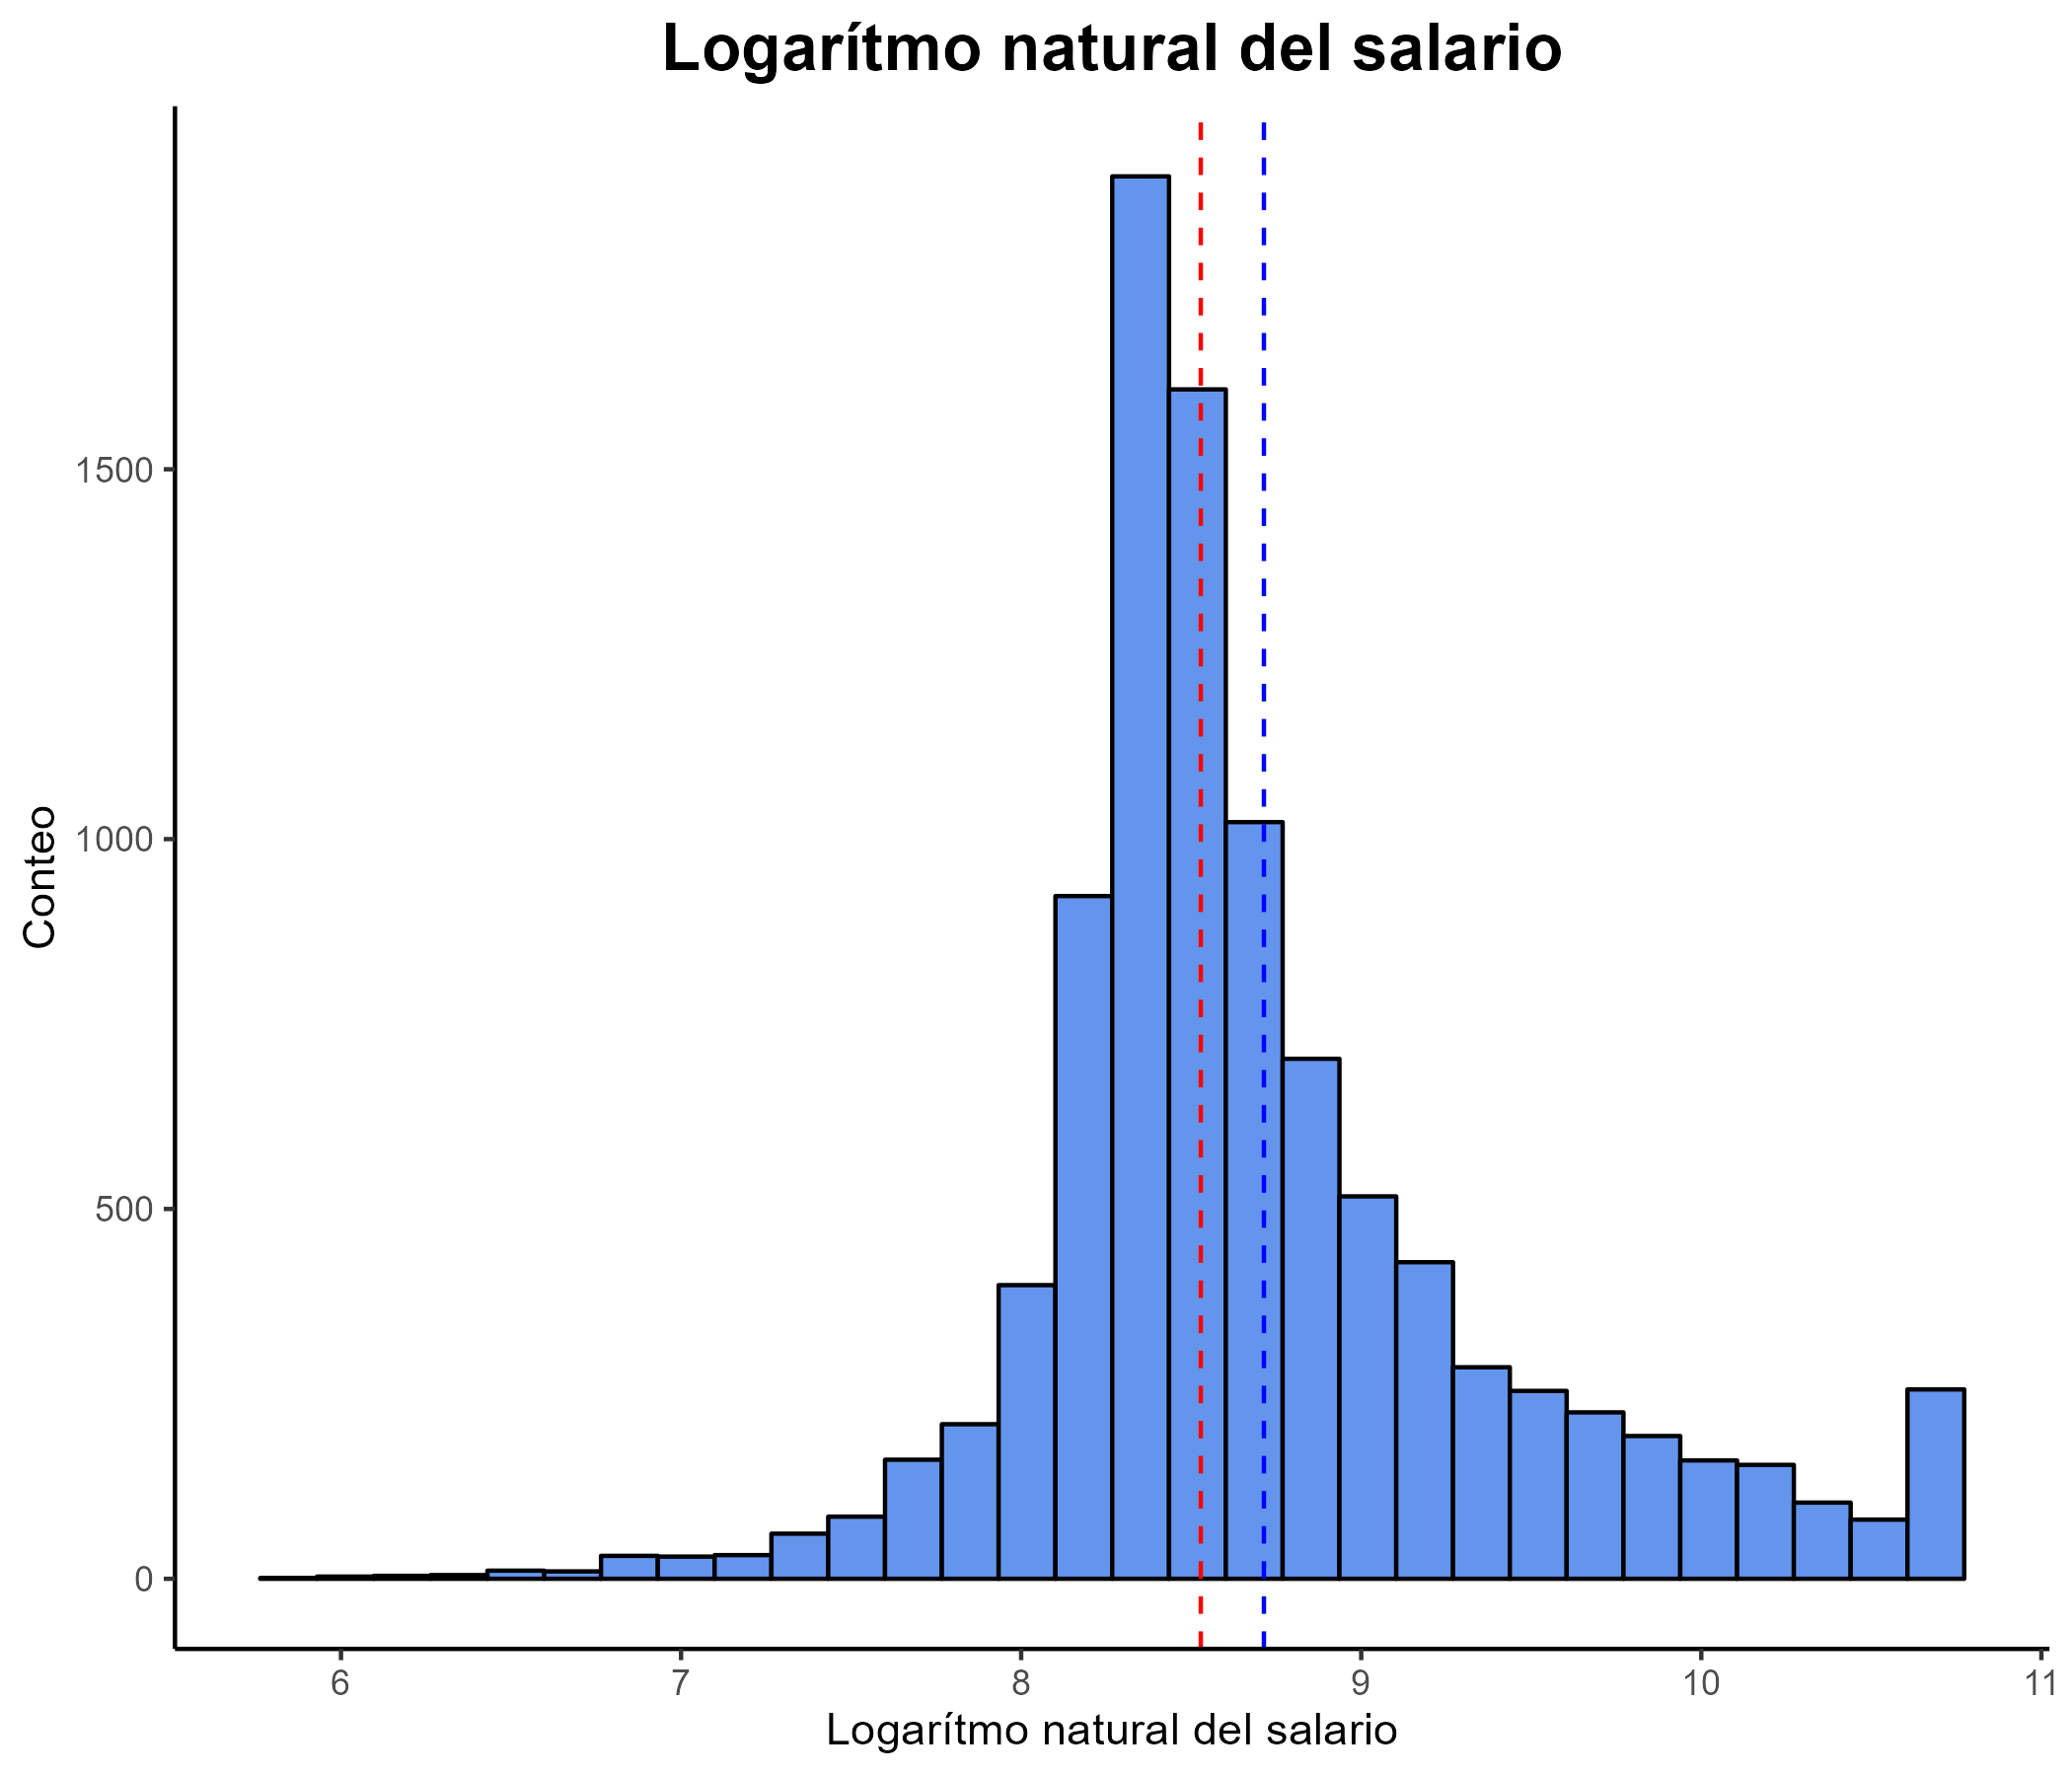
\includegraphics[width=0.45\textwidth]{Graficos/ln_sal.png}
    
    \label{fig:salarios}
    \par{\footnotesize{\textit{Nota:} En el panel izquierdo se encuentra la distribución del salario por hora en pesos. En el panel derecho se encuentra la distribución del logaritmo natural del salario por hora. La línea roja es la mediana de la variable mientras que la linea azul es la media.}}
\end{figure}
\newpage
\section{Perfilamiento del salario y la edad}

Con el fin de entender la relación entre la edad de un individuo y su salario, se estimó el modelo en la ecuación \ref{eq:modelo1}. 

\begin{equation}
    \ln{Salario_i} = \beta_0 + \beta_1 Edad_i + \beta_2 Edad^2_i + u_i
    \label{eq:modelo1}
\end{equation}

Los resultados de esta estimación se encuentran en la tabla \ref{modelo1tab}. En esta tabla se puede ver que tanto la edad como la edad al cuadrado tienen coeficientes que son estadísticamente significativos para explicar el logaritmo natural del salario. Además, se puede ver que la edad tiene un coeficiente positivo, mientras que el componente cuadrático tiene un coeficiente negativo.

\begin{table}[!htbp] 
\centering 
\caption{Resultados Modelo 1} 
\label{modelo1tab} 
\resizebox{0.6\textwidth}{!}{ % Ajusta el tamaño de la tabla
\begin{tabular}{@{\extracolsep{5pt}}lc} 
\\[-1.8ex]\hline 
\hline \\[-1.8ex] 
 & \multicolumn{1}{c}{\textit{Variable dependiente:}} \\ 
\cline{2-2} 
\\[-1.8ex] & ln(Salario) \\ 
\hline \\[-1.8ex] 
 Edad & 0.071$^{***}$ \\ 
  & (0.004) \\ 
  & \\ 
 Edad$^{2}$ & $-$0.001$^{***}$ \\ 
  & (0.00005) \\ 
  & \\ 
 Constante & 7.315$^{***}$ \\ 
  & (0.067) \\ 
  & \\ 
\hline \\[-1.8ex] 
Observaciones & 9,848 \\ 
R$^{2}$ & 0.047 \\ 
R$^{2}$ Ajustado& 0.047 \\ 
Error Estándar Residual& 0.676 (df = 9845) \\ 
\hline 
\hline \\[-1.8ex] 
\textit{Nota:}  & \multicolumn{1}{r}{$^{*}$p$<$0.1; $^{**}$p$<$0.05; $^{***}$p$<$0.01} \\ 
\end{tabular} 
}
\end{table}
Es importante destacar que estos coeficientes no pueden interpretarse de manera directa, ya que el efecto de la edad sobre el salario no es constante sino decreciente. Por lo tanto, para una interpretación adecuada, es necesario calcular el efecto marginal como se muestra en la ecuación \ref{efecto_marg} y evaluarlo en el valor promedio de la edad. Al realizar este procedimiento, hallamos que, para el individuo promedio, un aumento en un año de la edad aumenta el salario en 1.29\%, manteniendo todo lo demás constante.

\begin{equation}
    \frac{\partial \ln(Salario_i)}{\partial Edad} = \beta_1 + 2\beta_2 Edad
    \label{efecto_marg}
\end{equation}

Dado el efecto marginal decreciente de la edad sobre el salario, resulta relevante determinar la edad en la que el salario alcanza su valor máximo antes de comenzar a disminuir. Para determinar este punto, igualamos a cero la ecuación \ref{efecto_marg} y despejamos la edad. En otras palabras, aplicamos la condición de primer orden del problema de maximización del salario con respecto a la edad y encontramos la solución óptima. El resultado de este proceso se puede ver en la ecuación \ref{edad_pico}. Al evaluar esta ecuación en los valores encontrados en la tabla \ref{modelo1tab}, hallamos que, en promedio, el salario llega a su pico a los 44.23 años de edad del individuo.

\begin{equation}
    Edad_{pico} = -\frac{\beta_1}{2\beta_2}
    \label{edad_pico}
\end{equation}

Adicionalmente, por medio de la metodología de bootstrap hallamos el error estándar de 0.55 de la edad pico del salario. Gracias a esto podemos afirmar que, con un 95\% de confianza, la edad pico del salario se encuentra entre 43.17 y 45.32 años de edad. 
\\
\\
Finalmente, en la figura 2 se puede observar la relación entre el logaritmo natural del salario y la edad. En azul se pueden ver los datos observados, mientras que la línea roja representa la predicción a partir de la estimación de la tabla \ref{modelo1tab}. En esta figura se puede observar que el salario aumenta a medida que aumenta la edad, hasta que, alrededor de los 44 años de edad el salario alcanza un valor máximo y empieza a disminuir.  Esto se explica ya que a partir de la edad pico hay una combinación de factores, como de menor capacidad de aprendizaje, posible obsolescencia de habilidades, reducción de esfuerzo, discriminación y menor movilidad laboral hace que los salarios comiencen a disminuir. Este fenómeno es un reflejo de la interacción entre la oferta y demanda de trabajo, las decisiones individuales de los trabajadores y las políticas salariales de las empresas.


\begin{figure}[h]
    \centering
    \caption{Perfilamiento del salario contra la edad}
    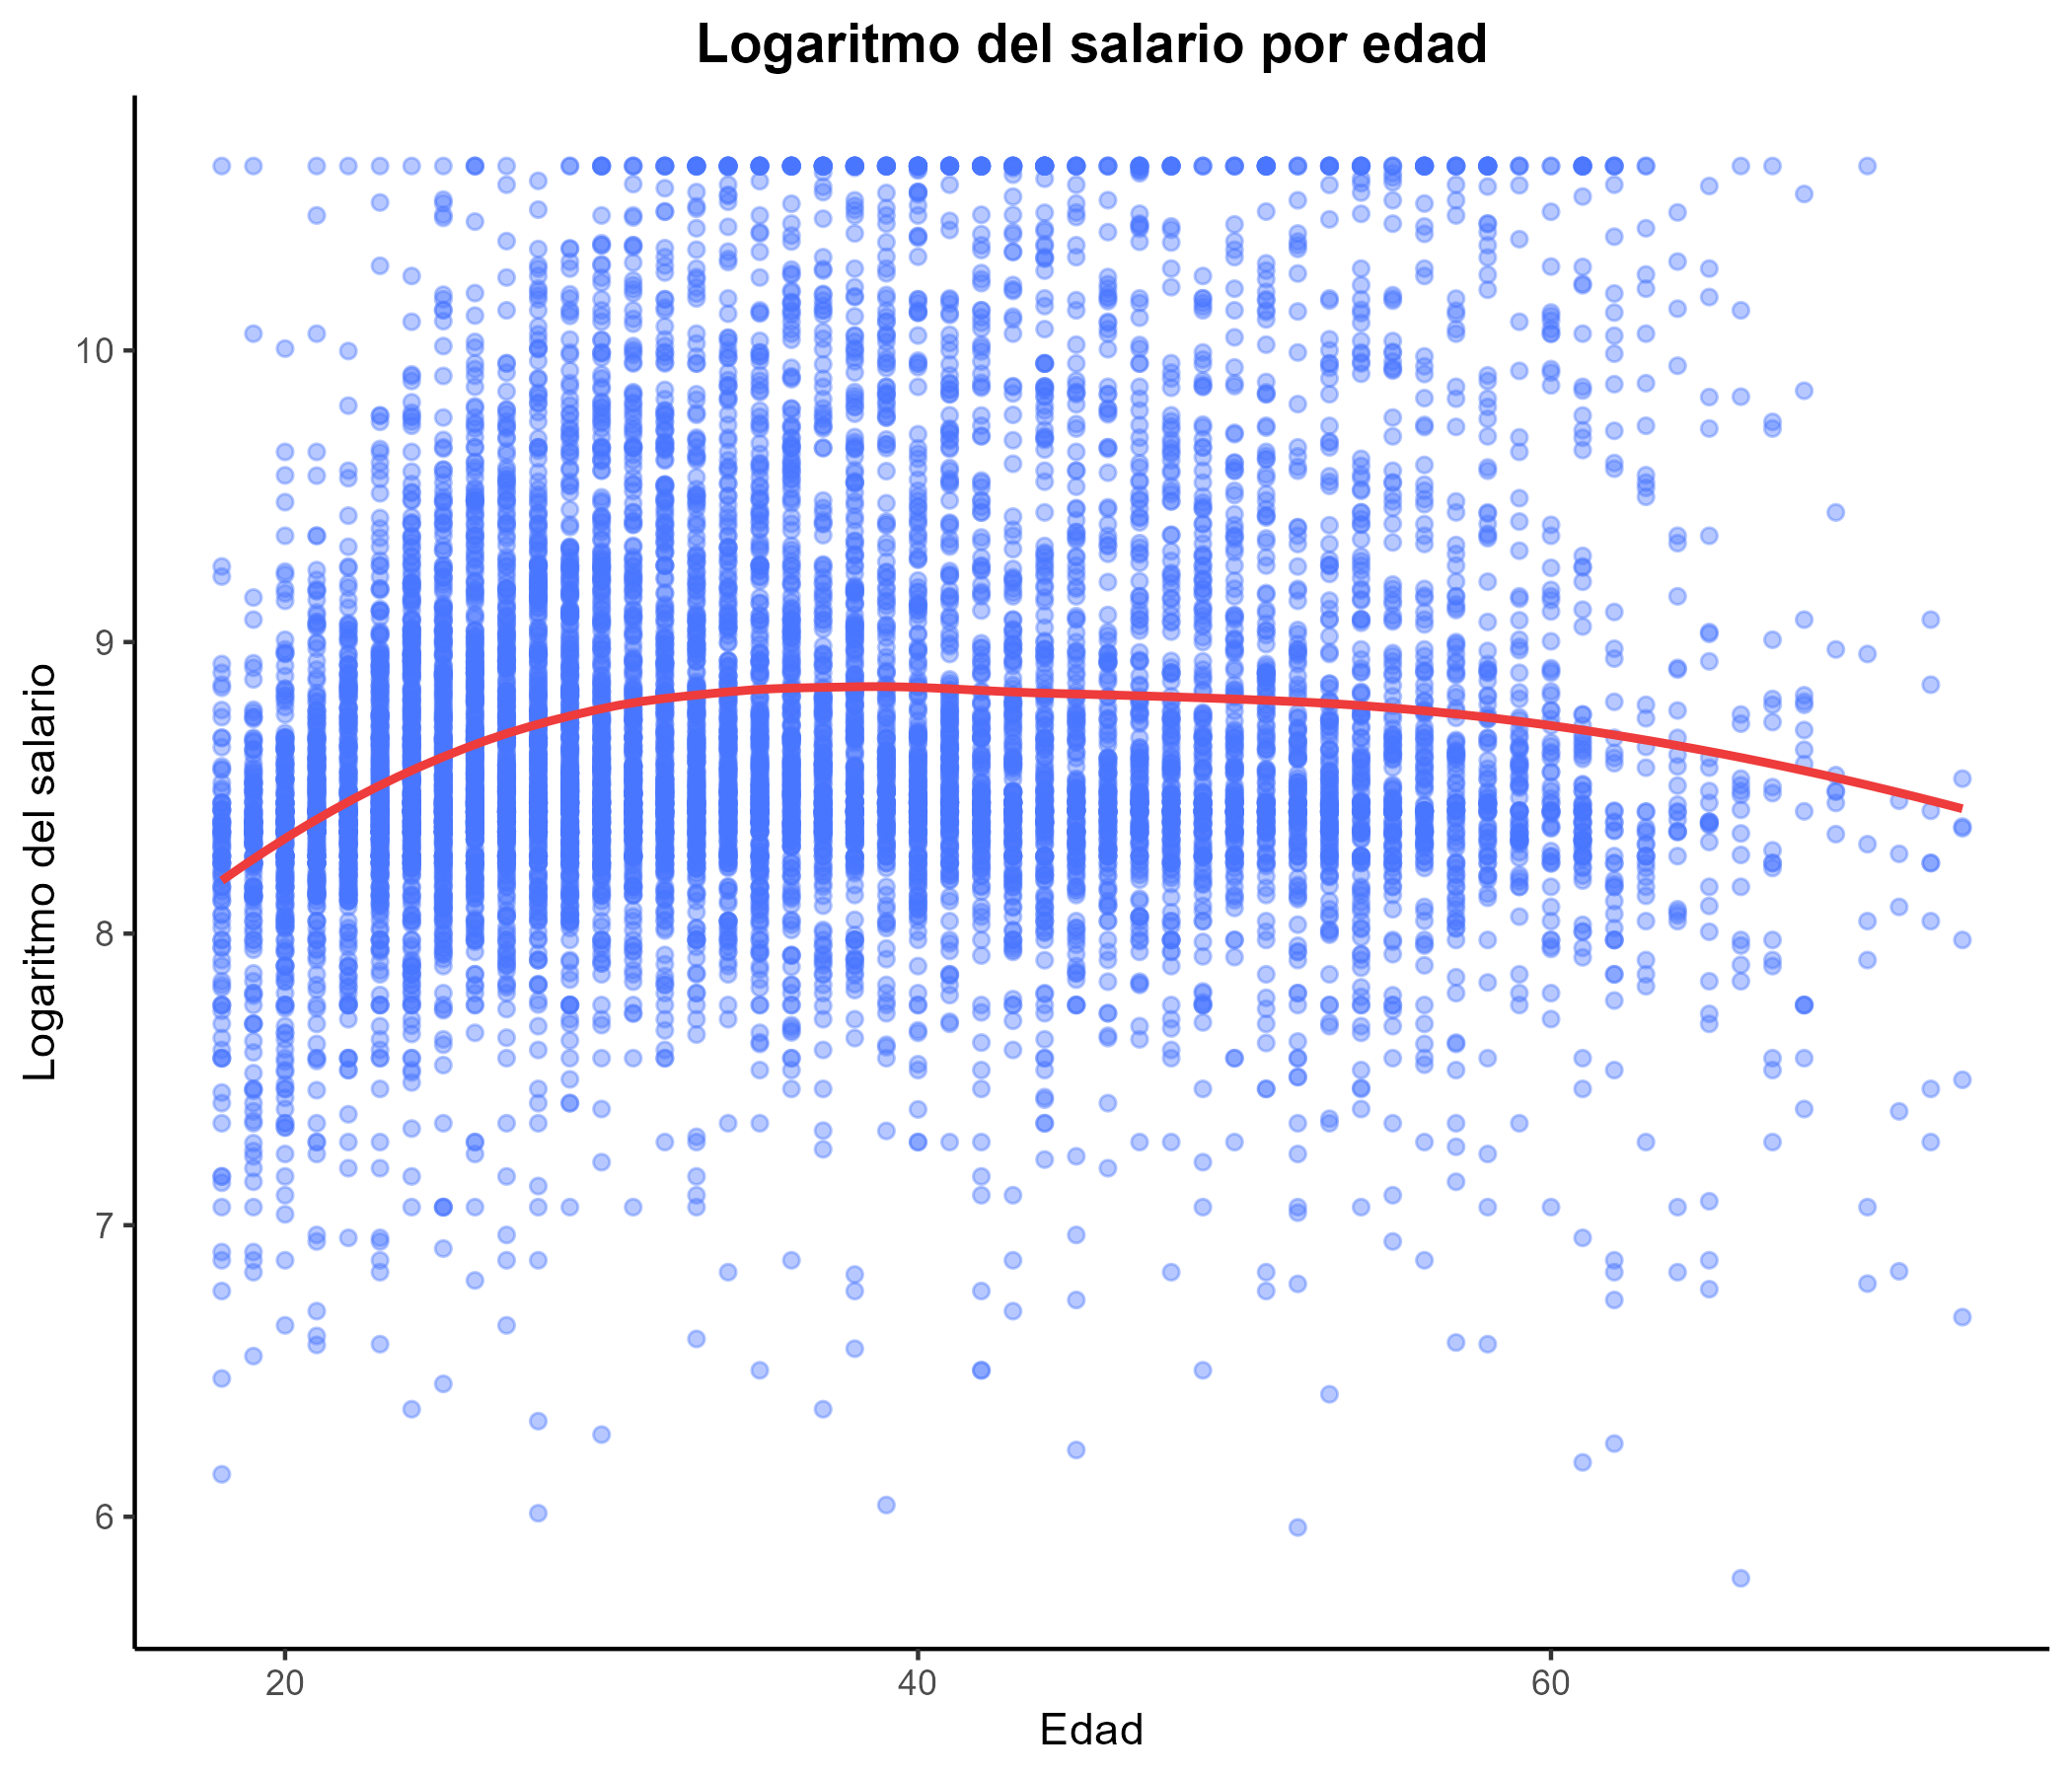
\includegraphics[width=0.6\textwidth]{Graficos/salario_por_edad_scatter.png}
    \label{fig:salario_edad}
\end{figure}


\newpage
\section{Brecha salarial de género}

\subsection{Presentación y Justificación del modelo}

Con la brecha salarial de género nos preguntamos ¿Las mujeres ganan menos salario por el hecho de ser mujeres? Para aproximarnos a esta pregunta es importante controlar por características productivas relevantes que influyen en el salario. Tradicionalmente, los economistas se han enfocado en: (i) el nivel de escolaridad, (ii) la industria, (iii) su oficio, (iv) y el tamaño de la firma, Blau & Kahn (2017) y Goldin et al. (2017). Adicionalmente, características como (v) el estado civil, (vi) el número de hijos y (vii) la edad son importantes porque están relacionada con decisiones de fertilidad y de cuidado que usualmente recaen sobre las mujeres, Barford et al. (2024). En este contexto (viii) las amenidades domésticas a las que tienen acceso las mujeres también influyen en sus decisiones de participación en el mercado laboral (ej. sí en la casa hay una lavadora las mujeres no tienen que usar todo el día para lavar ropa)
\\
\\
Teniendo en cuenta lo anterior se decidió incorporar en el modelo como variables de control: el nivel educativo (compuesta por 6 categorías donde 1 corresponde a sin educación y 7 a educación terciaria), tamaño de la firma (compuesta por 5 categorías donde 1 corresponde a cuenta propia y 5 a empresa con más de 50 personas), oficio (compuesta por 66 categorías una por ocupación) y formalidad (indicador de sector formal) para controlar por los conocimientos y las habilidades de las personas. Además, se incluyeron la edad y el estrato (compuesta por 6 categorías correspondientes a los estratos de Bogotá) como una forma de controlar por la etapa de las vida de las mujeres (si es probable que tengan hijos) y para medir si cuenta con amenidades domésticas. La variable predicha es el salario por hora y el predictor de interés es el indicador de género. 
    \begin{equation}
    \begin{split}
    \ln(Salario_i) &= \beta_0 + \beta_1 Mujer_i + \beta_2 NivelEduc_i + \beta_3 Edad_i + \beta_4 Edad^2_i  \\
    &\quad + \beta_5 TamañoFirma_i + \beta_6 Formal_i + \beta_7 Oficio_i + \beta_8 Estrato_i + u_i
    \end{split}
    \end{equation}

\vspace{2mm}

\subsection{Resultados}

\begin{table}[!htbp] \centering 
  \caption{Brecha salarial por género} 
  \label{} 
\resizebox{0.8\textwidth}{!}{ 
\begin{tabular}{@{\extracolsep{5pt}}lcccc} 
\\[-1.8ex]\hline 
\hline \\[-1.8ex] 
 & Sin condicionar & Condicionada & FWL & FWL Boot SE \\ 
\\[-1.8ex] & (1) & (2) & (3) & (4)\\ 
\hline \\[-1.8ex] 
 Mujer & $-$0.042 & $-$0.074 & $-$0.074 & $-$0.074 \\ 
  & (0.014) & (0.011) & (0.010) & (0.015) \\ 
  & & & & \\ 
\hline \\[-1.8ex] 
Observaciones & 9,848 & 9,848 & 9,848 & 9,848 \\ 
R$^{2}$ ajustado & 0.001 & 0.609 & 0.005 & 0.005 \\ 
EE Residual & 0.692 (df = 9846) & 0.433 (df = 9765) & 0.431 (df = 9846) & 0.431 (df = 9846) \\ 
\hline 
\hline \\[-1.8ex] 
\multicolumn{5}{c}{\textit{Nota: los modelos (2), (3) y (4) fueron estimados con los controles:}} \\
\multicolumn{5}{c}{\textit{Nivel de educación, Tamaño de la firma, Oficio, Sector formal, Estrato y Edad}} \\
\multicolumn{5}{c}{\textit{Estos controles fueron descritos en la sección 4.1 }} \\
\end{tabular} 
}
\end{table} 


Según los cuatro modelos estimados las mujeres ganan un salario menor con respecto a los hombres. Respectivamente, (-4,2\%) según el primer modelo  y (-7,4\%) de acuerdo con los demás. Para todos los casos los coeficientes estimados son significativos estadísticamente y prácticamente es llamativo que una característica no relacionada con la productividad afecte el salario. Entre los cuatro modelos el que mejor se ajusta a los datos dentro de la muestra es el segundo modelo (media condicionada) que cuenta con más información para estimar el salario en contraste con los otros modelos que solo cuentan con una variable. 
\\
\\
Es importante resaltar que comparando los modelos tres y cuatro los errores estándar del modelo cuatro, que fueron calculados por medio de bootstrapping son más grandes que los estimados en el modelo tres. Esto sucede porque los errores estándar del modelo tres fueron calculados de manera predeterminada por R asumiendo condiciones de Gauss-Markov y por ende una menor variación en los residuales. En contraste, los errores estándares del modelo cuatro calculados por bootstrapping usan al variación de la muestra original para generar variación sintética y aproximarse a la distribución muestral del coeficiente de género si asumirla. 
\\
\\
Estos resultados indican que hay una relación entre el hecho de ser mujer y percibir un menor salario. Entre las explicaciones para esta relación resaltan la carga desproporcionada que reciben las mujeres de la economía del cuidado (selección no voluntaria a la labores del cuidado) Barford et al. (2025)  y la penalización por la maternidad (selección de las mujeres por fuera del mercado laboral para cuidar a sus hijos) Kleven et al. (2021). Adicionalmente, también puede haber discriminación contra las mujeres en edad de tomar sus decisiones de fertilidad (los discriminadores no contratan mujeres en edad de quedar embarazadas para no cubrir licencias de maternidad). Los tres casos aquí expuestos pretenden convencer al lector de que la brecha salarial de género tiene un componente tanto de selección como de discriminación. Es importante notar que hay más mecanismo que puede explicar la brecha.

\subsection{Perfil de salario por edad y género}

\begin{figure}[H]
    \centering
    \caption{Perfil de salario por edad y género}
    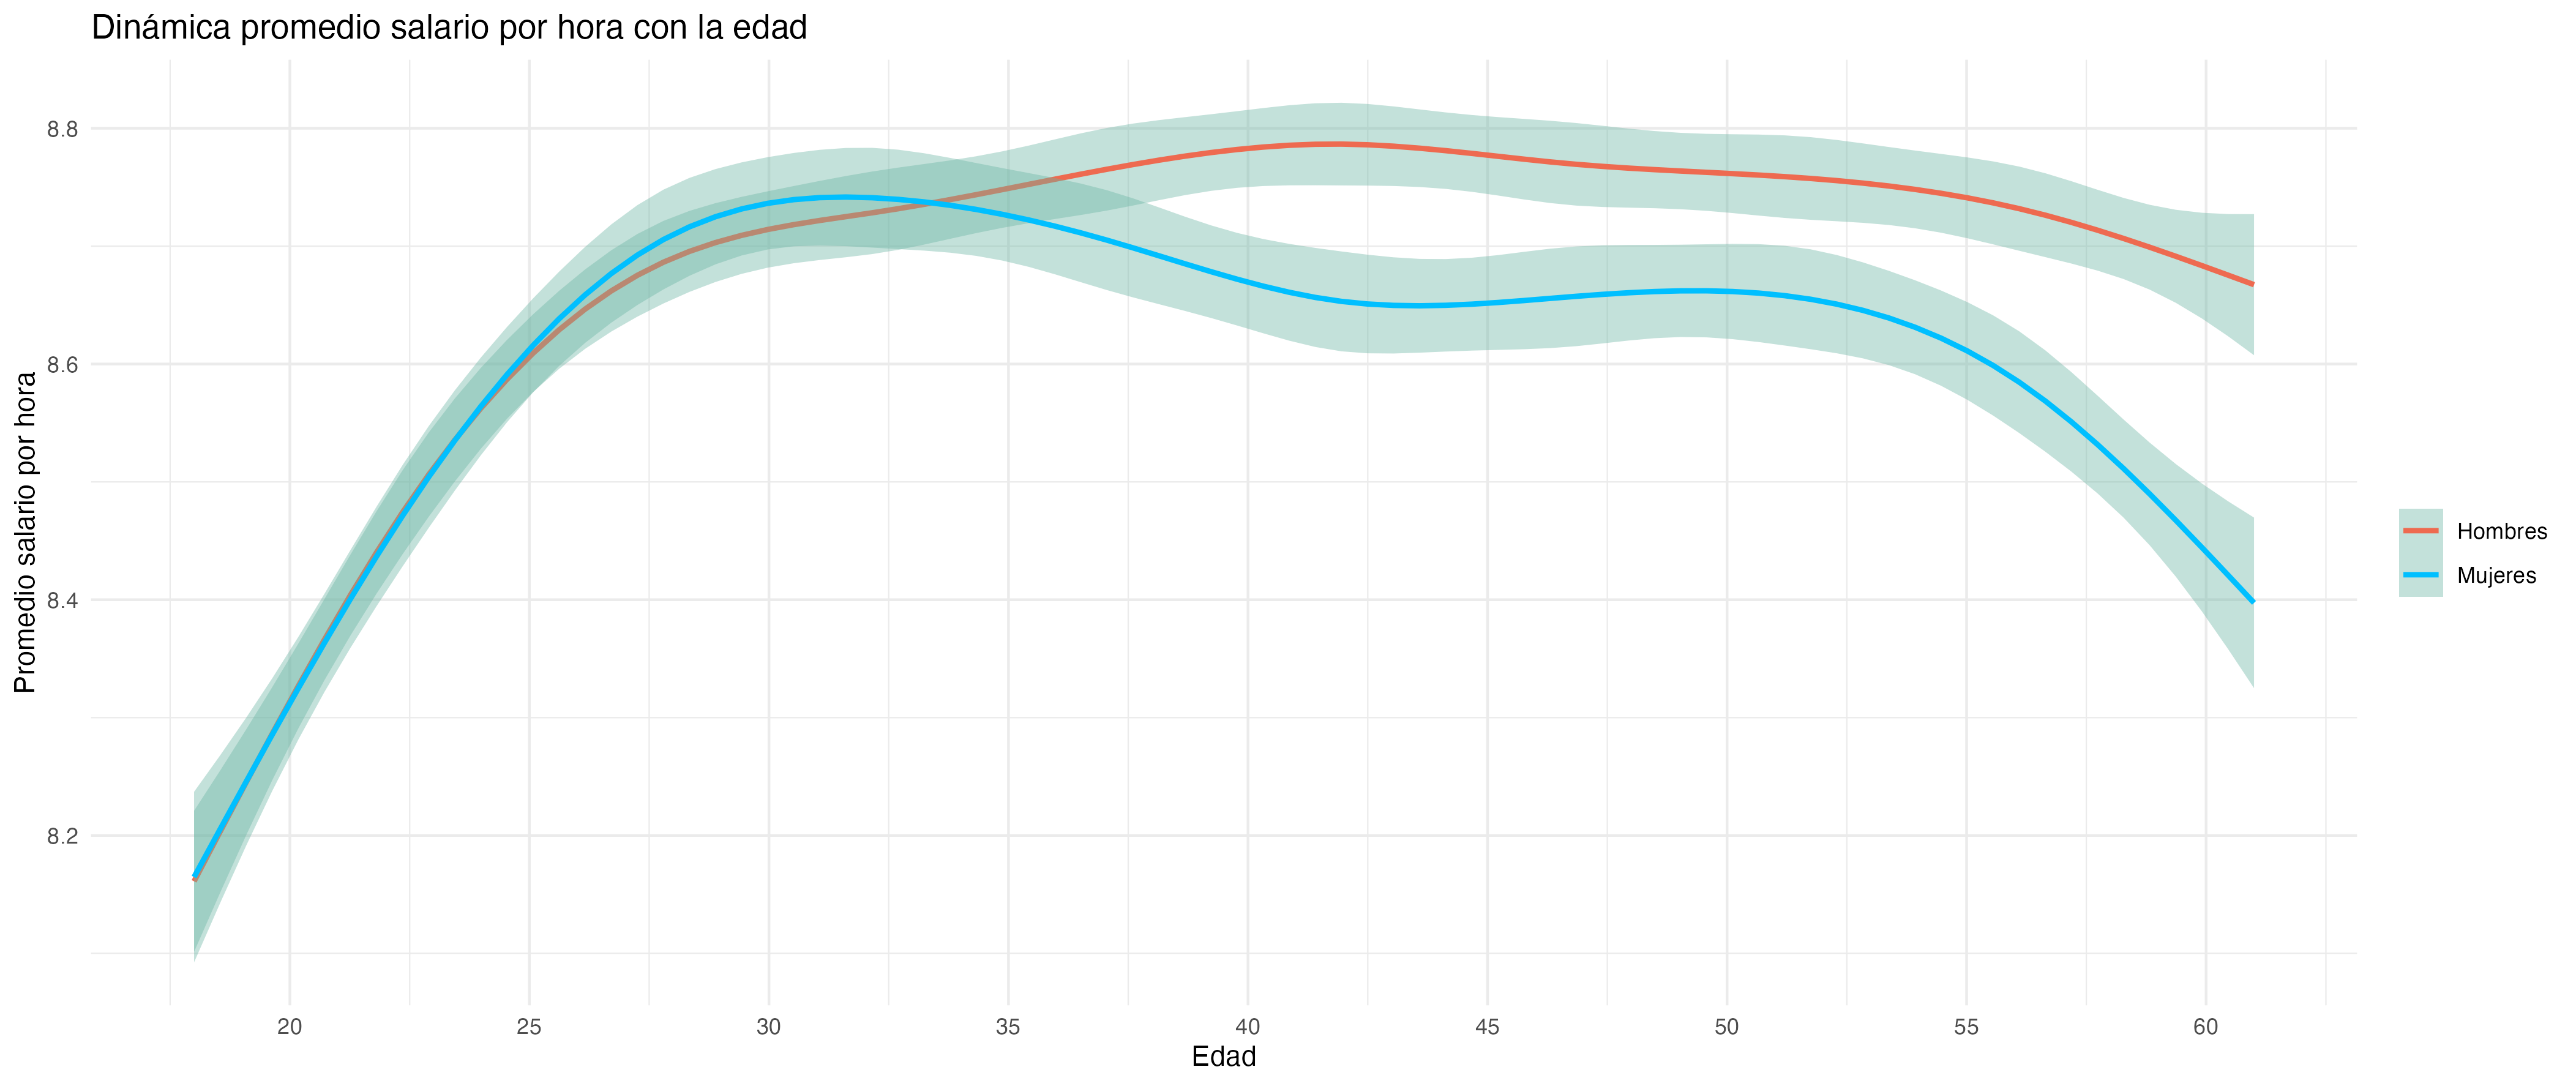
\includegraphics[width=0.8849\linewidth]{Graficos/dinamica_promedio_salario_por_hora_con_la_edad.png}
    \label{fig:enter-label}
\end{figure}

Según el DANE (2019) alrededor del 50\% de las mujeres que deciden ser madres tienen su primer hijo entre los 20 y los 29 años. Esto podría explicar la forma de “M” que se puede evidenciar en la gráfica del perfil de salario por edad para las mujeres. La gráfica llega a su punto máximo a alrededor de los 30 años, luego presenta un descenso que podría ser explicado por la salida de las mujeres del mercado laboral para cuidar de sus hijos y finalmente vuelve a subir cuando las mujeres se han reincorporado al mercado laboral. En contraste, el perfil de salario por edad de los hombres sube hasta que alrededor de los 40 años y tiende a quedarse allí.  Estas estimaciones tienen un incertidumbre de aproximadamente 2 años para las mujeres y aproximadamente de 2.4 años para los hombres. Con medias centradas en 49 años para las mujeres y 53 para los hombres. 
Consideramos que estos resultados difieren de las tendencia presentadas en el gráfico por dos razones, (i) el gráfico se limpió con el fin de remover valores atípicos y años con pocas observaciones, (ii) la continuidad que tienen los picos de edad salario entre sí. Con respecto a la explicación inicial sobre el comportamiento de la curva de las mujeres, las estimaciones de la edad pico indican que la primera subida salarial es más pequeña que la segunda (donde aparece el pico) a diferencia del gráfico.

\section{Predicción del ingreso}

Para mayor facilidad, vamos a dividir algunas variables explicativas en las siguientes categorías:
Los ingresos pueden clasificarse en varias categorías. Los \textbf{ingresos laborales} incluyen el ingreso por primas, bonificaciones y el ingreso laboral secundario. Los \textbf{subsidios} comprenden el subsidio de alimentación, transporte, familiar y educativo. Los \textbf{ingresos en especie} abarcan el valor de los alimentos, vivienda, transporte y otros beneficios no monetarios. Las \textbf{primas y bonificaciones adicionales} incluyen la prima por servicios, navidad y vacaciones, así como viáticos y bonificaciones anuales. Finalmente, los \textbf{ingresos no laborales} provienen de diversas fuentes como arriendos, pensiones, pensión alimenticia, transferencias de otros hogares dentro y fuera del país, ayudas institucionales, dividendos, cesantías y otras fuentes de ingreso.


En primera instancia se dividió la muestra en dos partes, un 70\% para entrenamiento y un 30\% para testeo. Los modelos, su especificación y desempeño bajo este modelo de Validation Set se mencionan a continuación.

\subsection{Modelos previos}

Los modelos previos están expuestos en las secciones anteriores, siendo el primer modelo la fórmula (1), el segundo modelo tiene únicamente como variable independiente si el individuo es hombre o mujer y el tercer modelo expresado en la fórmula (4).
\\
\\
El primer modelo recoge una parte importante en la predicción, pero deja por fuera muchas otras variables que explican este ingreso laboral. El segundo únicamente como variable independiente si el individuo es hombre o mujer. La intención de este modelo es recoger la influencia de las brechas de género en el ingreso laboral. Así como el modelo anterior, este deja por fuera muchas variables influyentes en el ingreso.
Finalmente, el modelo agrupa muchas más variables relevantes que los modelos anteriores y agrega flexibilidad elevando la edad al cuadrado, aumentando la complejidad y de esta manera aumentando la certeza de la estimación con los datos de entrenamiento.

\subsection{Nuevos modelos}
    
\textbf{Modelo 4}

\footnotesize
\begin{equation}
    \begin{aligned}
        \ln(Salario_i) &= \beta_0 + \beta_1 Mujer_i + \beta_2 NivelEduc_i + \beta_3 Edad_i + \beta_4 Edad_i^2  + \beta_5 TamañoFirma_i + \beta_6 Formal_i  + \beta_7 Oficio_i \\ 
        &\quad  + \beta_8 Estrato_i + \beta_9 ExperienciaPot_i + \beta_{10} ExperienciaPot_i^2 + \beta_{11} HorasTrabajadas_i+ u_i
    \end{aligned}
\end{equation}

\normalsize
\\
Este modelo compone las variables del modelo anterior más la inclusión de una variable de experiencia potencial con su potencia al cuadrado, y una variable del total de horas trabajadas semanalmente. Estas transformaciones flexibilizan la predicción para acomodarse aún más a los datos de entrenamiento y así disminuir el sesgo.
\\
\textbf{Modelo 5}

\footnotesize
\begin{equation}
\begin{array}{l}
\ln(Salario_i) = \beta_0 + \beta_1 (Mujer_i \ast ParentescoJefe_i) 
+ \sum_{j=1}^{4} \beta_{1+j} (Edad_i^j \ast NivelEduc_i) 
+ \beta_6 (TamañoFirma_i \ast Formal_i) \\ 
+ \beta_7 Oficio_i + \beta_8 Estrato_i 
+ \sum_{j=1}^{4} \beta_{8+j} ExperienciaPot_i^j 
+ \beta_{13} HorasTrabajadas_i + u_i
\end{array}
\end{equation}
\normalsize
\\
Este modelo incluye interacciones entre las variables del modelo anterior y aumenta el grado de los polinomios a cuatro en las variables de edad y experiencia potencial. El resultado de este modelo es el mismo del modelo anterior, disminuyendo el RMSE aumentando el ajuste a los datos de entrenamiento.
\\
\textbf{Modelo 6}

\footnotesize
\begin{equation}
\begin{array}{l}
\ln(Salario_i) = \beta_0 + \beta_1 (Mujer_i \ast ParentescoJefe_i) 
+ \sum_{j=1}^{4} \beta_{1+j} (Edad_i^j \ast NivelEduc_i) \\
+ \beta_6 (TamañoFirma_i \ast Formal_i) + \beta_7 Oficio_i + \beta_8 Estrato_i 
+ \sum_{j=1}^{4} \beta_{8+j} ExperienciaPot_i^j + \beta_{13} HorasTrabajadas_i \\
+ \beta_{14} Subsidios_i + \beta_{15}PrimasBonificaciones_i + u
\end{array}
\end{equation}
\normalsize
\\
Este modelo incorpora variables relacionadas con los subsidios, así como las primas y bonificaciones otorgadas a los individuos. La inclusión de estas variables incrementa nuevamente el ajuste del modelo, lo que resulta en el modelo más equilibrado entre el sesgo y la varianza en las predicciones.
\\
\textbf{Modelo 7}
\\
\footnotesize
\begin{equation}
\begin{array}{l}
\ln(w) = \beta_0 + \beta_1 Mujer_i \ast ParentescoJefe_i 
+ \sum_{n=1}^{4} \beta_{1+n} Edad_i^n \ast NivelEduc_i \\
+ \beta_6 TamañoFirma_i \ast Formal_i + \beta_7 Oficio_i + \beta_8 Estrato_i 
+ \sum_{n=1}^{4} \beta_{8+n} ExperienciaPot_i^n \ast HorasTrabajadas_i^n) \\
+ Subsidios_i + PrimasyBonificaciones_i + {IngresosLaborales_i 
+ IngresosNoLaborales_i + IngresosEnEspecie_i + u
\end{array}
\end{equation}
\normalsize
\\
Este modelo añade un polinomio de las horas trabajadas y la interacciona con el polinomio de la experiencia potencial, adicionalmente, añade los ingresos laborales, no laborales y en especie. El resultado de este modelo es un sobreajuste a los datos de entrenamiento que es castigado por la varianza respecto a los datos de testeo.
\\
\textbf{Modelo 8}
\\
\footnotesize
\begin{equation}
\begin{array}{l}
\ln(w_i) = \beta_0 + \beta_1 (\text{Female}_i \ast \text{ParentescoJefe}_i) 
+ \sum_{j=1}^{8} \beta_{1+j} (\text{Age}_i^j \ast \text{NivelEduc}_i) + \beta_9 (\text{SizeFirm}_i \ast \text{Formal}_i) \\
 + \beta_{10} \text{Oficio}_i + \beta_{11} \text{Estrato}_i 
+ \sum_{j=1}^{8} \beta_{11+j} (\text{ExperienciaPot}_i^j \ast \text{HorasTrabajadas}_i^j) + \beta_{20} \text{Subsidios}_i \\
+ \beta_{21} \text{PrimasBonificaciones}_i + \beta_{22} \text{IngresosLaborales}_i 
+ \beta_{23} \text{IngresosNoLaborales}_i + \beta_{24} \text{IngresosEnEspecie}_i + u_i
\end{array}
\end{equation}
\normalsize
\\
El último modelo solo añade complejidad por medio del aumento del grado de los polinomios, pasándolos de cuarto a octavo grado. Este es el modelo con mayor error de predicción explicado por el sobreajuste de la predicción a los datos de entrenamiento.
\\
\subsection{Resultados}

\begin{figure}[h]
    \centering
    \begin{minipage}{0.5\textwidth}  % Ajusta el ancho según necesites
        \centering
        \caption{Desempeño de los modelos con validation set}
        \includegraphics[width=\linewidth]{Graficos/Desempeño_validation_set.png}
        \label{fig:Errores}
    \end{minipage}%
    \begin{minipage}{0.5\textwidth}  % Ajusta el ancho para la tabla
        \centering
        \begin{tabular}{@{\extracolsep{5pt}} ccc} 
        \hline 
        Modelo & RMSE \\ 
        \hline 
        $1$ & $0.6731$ \\ 
        $2$ & $0.6880$ \\ 
        $3$ & $0.4344$ \\ 
        $4$ & $0.4051$ \\ 
        $5$ & $0.3962$ \\ 
        $6$ & $0.3664$ \\ 
        $7$ & $0.3932$ \\ 
        $8$ & $0.7783$ \\ 
        \hline 
        \end{tabular}  
    \end{minipage}
\end{figure}


Los modelos se construyeron desde el más simple hasta el más complejo. El análisis del RMSE reveló un comportamiento cóncavo, con los mayores errores en el segundo y el último modelo. Se observaron dos saltos significativos en el desempeño: entre los modelos dos y tres, y entre los modelos siete y ocho. La primera mejora se debe a la incorporación de variables relevantes, mientras que la segunda se explica por el aumento en el grado de los polinomios, que pasa de cuatro a ocho.
\\
\\
El modelo con mejor desempeño fue el número seis, este modelo se diferencia del cinco por la inclusión de variables como subsidios, primas y bonificaciones, y del siete por la omisión de la interacción entre la experiencia potencial y las horas trabajadas, además de una nueva interacción entre los polinomios de cuarto orden de la experiencia potencial y el total de horas trabajadas.
\\
\\
El éxito del modelo se debe al uso moderado de polinomios y a la exclusión de variables de ingreso laboral y no laboral. Un grado moderado en los polinomios evita un sobreajuste a los datos de entrenamiento, reduciendo la varianza en la muestra de prueba. Por su parte, las variables de ingreso laboral y no laboral aportan tanta información que facilitan una predicción precisa en la muestra de entrenamiento, pero pueden comprometer la generalización del modelo.

\subsection{Outliers}

\begin{figure}[h]
    \centering
    \caption{Distribución de los errores de predicción del modelo con mejor desempeño}
    \includegraphics[width=0.6\textwidth]{Graficos/Distribucion_errores.png}    
    \label{fig:Errores}
    
    \vspace{0.1cm} % Espacio opcional para separar la nota
    \footnotesize Nota: Las líneas verticales de color verde representan el límite de tres desviaciones estándar.
\end{figure}

Para identificar los outliers por medio de los errores del modelo con mejor desempeño, se seleccionaron las observaciones cuyos errores se ubicaban fuera del rango intercuartílico (0,25 y 0,75). Al analizar las características de estos outliers, no se detectaron anomalías significativas en sus distribuciones. Sin embargo, al ajustar el rango a las observaciones que están a más de tres desviaciones estándar se observó que estas observaciones contaban con una mayor proporción de trabajadores informales. Esto sugiere que el modelo presenta ciertas dificultades para predecir con precisión los ingresos de los trabajadores informales, posiblemente debido a la falta de información representativa o a sesgos inherentes a la naturaleza del trabajo informal. Esta limitación indica que los trabajadores informales podrían requerir un tratamiento diferenciado en el modelo, ya sea mediante la incorporación de variables adicionales o técnicas específicas que capturen mejor las particularidades de este grupo.

\subsection{Leave one out cross validation}

El desempeño de los modelos bajo el método de LOOCV no difirió significativamente en ninguno de los casos, e incluso mejoró para el modelo 7. Esto sugiere que la partición del validation set no fue determinante en el desempeño de los modelos, ya que estos se comportaron de manera consistente en ambas aproximaciones. Es importante destacar que este análisis se centra en los modelos 6 y 7. Al realizar pruebas bajo la aproximación de K-fold con $k=10$, el desempeño de estos dos modelos no mostró grandes variaciones respecto al validation set. Sin embargo, el modelo con peor desempeño en el validation set sí presentó cambios significativos. A partir de esta revisión, se evidencia la falta de rigurosidad en el testeo mediante un validation set como método único de evaluación. En este sentido, el modelo 6 presenta valores de RMSE de 0.366 en validación simple y LOOCV, y 0.367 en $k$-fold. El modelo 7 tiene un RMSE de 0.393 en validación simple, 0.366 en LOOCV y 0.372 en $k$-fold. Finalmente, el modelo 8 muestra un RMSE de 0.778 en validación simple y 0.424 en $k$-fold, sin valor reportado para LOOCV.

\bigskip

Por otro lado, el estadístico de influencia se relaciona al error de predicción de LOOCV por medio del efecto que tiene omitir una observación en los valores predichos por el modelo. Dado que la expresión del Cross Validation tiene en el numerador el error de predicción y en el denominador 1 menos el leverage de la variable, un nivel de leverage alto tiene que ser compensado de manera proporcional por un bajo valor del error de predicción. Este comportamiento se ve en los modelos, con el leverage promedio más alto en los modelos con menor error de predicción.

\begin{thebibliography}{99} %% use BibTeX or add references manually


\bibitem{ilo2025}
Barford et al. (2025)
\emph{VOLUNTEERING, UNPAID CARE WORK AND GENDER IN LOWER-INCOME COUNTRIES}, 
\emph{United Nations Voluteers (UNV) and International Labor Organization (ILO)}
https://www.ilo.org/sites/default/files/2025-02/57956-UNV-ILO-Publication-FINAL-v3-WEB.pdf 

\

\bibitem{bordot2022}
Bordot, F. (2022).
\emph{Artificial intelligence, robots and unemployment: Evidence from OECD countries}.
\emph{Journal of Innovation Economics \& Management}, (1), 117-138.

\

\bibitem{blau2017}
Blau, F. D., & Kahn, L. M. (2017)
\emph{The gender wage gap: Extent, trends, & explanation}.
\emph{Journal of Economic Literature}, 55(3), 789–865.
https://doi.org/10.1257/jel.20160995


\

\bibitem{casas2024}
Casas, L. (16 de septiembre de 2024)
\emph{Colombia suma más de 10 reformas tributarias en los últimos 20 y cuatro gobiernos}.
\emph{La República},
https://www.larepublica.co/especiales/reforma-tributaria-2024/colombia-suma-mas-de-10-reformas-tributarias-en-ultimos-20-anos-y-cuatro-gobiernos-3952802#:~:text=En\%20concreto\%2C\%20en\%20los\%20últimos,presentado\%20por\%20el\%20Gobierno\%20
Nacional.



\

\bibitem{chivu2022macroeconomic}
Chivu, S. I. (2022).
\emph{The Macroeconomic Impact of Artificial Intelligence}.
\emph{International Journal of Sustainable Economies Management},
vol. 13, no. 1, pp. 1--20.
doi: \href{https://doi.org/10.21511/ijsem.22(1).2022.01}{10.21511/ijsem.22(1).2022.01}.



\

\bibitem{Dane2019}
DANE (12 de mayo de 2019).
\emph{Dinámica edad en las que las mujeres tienen su primer hijo}.
\emph{X (antes Twitter)},
\text{https://x.com/DANE_Colombia/status/1127632693200588800}


\

\bibitem{goldin2017}
Goldin et al. (2017)
\emph{The expanding gender earnings gap: Evidence from the LEHD-2000}.
\emph{American Economic Review}, 107(5), 110–114.
https://doi.org/10.1257/aer.p20171065

\

\bibitem{Mejía2022}
Mejía, L. (2022)
\emph{¿Qué hacer en política tributaria?}.
\emph{Fedesarrollo},
https://www.repository.fedesarrollo.org.co/handle/11445/4279

\

\bibitem{kleven2021}
Kleven, H., Landais, C., & Søgaard, J. E. (2021)
\emph{Does Biology Drive Child Penalties? Evidence from Biological and Adoptive Familie}.
\emph{American Economic Review: Insights}, 3(2), 183–198.
https://doi.org/10.1257/aeri.20200260




\end{thebibliography}

\end{document}

